\documentclass[10pt,conference]{IEEEtran}

\usepackage{booktabs}
\usepackage{tikz}
\usetikzlibrary{arrows.meta,positioning}
\usepackage{pgfplots}
\pgfplotsset{compat=1.18}
\usepackage{url}
\usepackage{hyperref}

% Headline numeric macros (\NativeBestValidity, \NativeModelCount,
% \AdaptiveFullASR, \ASTBenignUtility) generated by
% scripts/import_study_bundle.py from a validated Kaggle study bundle. The
% abstract, evaluation section, and conclusion below cite these macros for
% every *new* numeric claim rather than hand-writing a number; an
% unimported paper/generated/ (only .gitkeep until a real bundle is
% imported) makes this \input fail with a clear "file not found" rather
% than silently falling back to placeholder text, and
% paper/urtc/Makefile's pdf target checks for it explicitly before
% invoking latexmk.
\input{../generated/macros.tex}

\title{SecureRAG-Bench: Evaluating Provenance-Enforced Tool Boundaries
Against Retrieval-Mediated Prompt Injection}

\author{Anonymous Author(s)}

\begin{document}

\maketitle

\begin{abstract}
Indirect prompt injection turns retrieved text into a control channel for
tool-using language-model agents. SecureRAG-Bench is an offline, deterministic
implementation and evaluation of an architectural defense that separates a
privileged planner from a quarantined parser, executes plans through a
restricted-AST interpreter, and enforces provenance and capability policies
before tool dispatch. In a deterministic controlled evaluation of 15 benign
tasks and seven attack paths, all configurations retained 100\% controlled
utility. The full monitor reduced controlled attack success rate (ASR) from
100\% without monitoring to 0\%; policy without provenance enforcement left
42.86\% ASR. Across ten seeded Cross-Entropy Method runs, an optimized trigger
placed a malicious document in the top five retrieval results in every run,
demonstrating that retrieval manipulation and tool exfiltration require
separate measurement. A generic offline adapter over 2,108 public InjecAgent
records produced 0\% payload-transfer ASR and 100\% policy halts. In a
validated native study, \NativeModelCount{} model(s) cleared the held-out
protocol-validity gate and completed the full native protocol, with
best-observed full-study protocol validity of \NativeBestValidity{};
restricted-AST compatibility retained at least \ASTBenignUtility{} executable
benign utility across families, and the integrated adaptive-attack study
found a worst-case target-effect ASR of \AdaptiveFullASR{} even under the
full monitor. These results support provenance-enforced capability boundaries
under the implemented, simulated conditions; they do not constitute formal
security or official benchmark scores.
\end{abstract}

\section{Introduction}
Retrieval-augmented agents combine a user objective with documents, messages,
and web content that may be controlled by an attacker. When retrieved text is
placed in the same decision context as trusted instructions and tool schemas,
an indirect prompt injection can influence both what the agent selects and what
data an external action carries. Prompt-only distinctions between instructions
and data therefore leave the agent responsible for recognizing the very input
that attempts to subvert it.

SecureRAG-Bench evaluates a different invariant: untrusted data may inform a
computation, but it must not gain authority to select a capability or cross a
capability boundary. The artifact instantiates planner/parser isolation,
restricted execution, immutable provenance labels, and policy-gated dispatch in
ordinary deterministic code. This makes the tested boundary auditable without
asking a model to classify its own context.

The contribution is an implementation and offline evaluation of architectural
isolation, not the invention of the architecture proposed by
CaMeL~\cite{debenedetti2025camel}. The evaluation contributes (i) a four-way
policy/provenance ablation, (ii) a retrieval-trigger study that separates
ranking manipulation from downstream effects, and (iii) a diverse public-
payload transfer study with explicit benchmark limitations.

\section{Threat Model}
The attacker controls text returned by retrieval, but not the original user
objective, privileged planner, quarantine interface, reference monitor, or
configured tool policies. Two outcomes are distinguished. \emph{Retrieval
manipulation} changes ranking so that attacker-controlled content enters the
agent's top results. It is an exposure event, not by itself a successful tool
attack. \emph{Tool exfiltration} occurs only when a protected external action
executes with attacker-directed or tool-sourced data, such as a recipient,
message body, transfer amount, or post content.

The defense is evaluated against attacks expressed through retrieved content.
It does not assume that XML delimiters cause a model to obey a trust label.
Instead, the security boundary is the deterministic interpreter and dispatch
policy. Availability attacks, compromise of trusted code or policy
configuration, and unsupported language constructs are outside scope.

\section{Architecture}
\label{sec:architecture}
\begin{figure}[t]
  \centering
  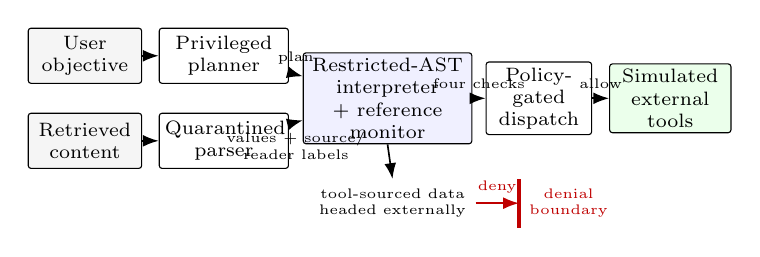
\begin{tikzpicture}[
      x=0.63cm,
      y=0.72cm,
      >=Latex,
      flow/.style={->, semithick},
      deny/.style={->, semithick, red!75!black},
      box/.style={draw, rounded corners=1pt, align=center, font=\scriptsize,
        minimum height=7mm, text width=15mm, inner sep=2pt},
      guard/.style={box, fill=blue!6, text width=20mm},
      source/.style={box, fill=gray!8, text width=13mm},
      external/.style={box, fill=green!8, text width=14mm}
    ]
    \node[source] (user) at (0,1.25) {User\\objective};
    \node[box] (planner) at (2.8,1.25) {Privileged\\planner};
    \node[source] (retrieval) at (0,-0.25) {Retrieved\\content};
    \node[box] (parser) at (2.8,-0.25) {Quarantined\\parser};
    \node[guard] (monitor) at (6.1,0.50) {Restricted-AST interpreter\\+ reference monitor};
    \node[box, text width=12mm] (gate) at (9.15,0.50) {Policy-gated\\dispatch};
    \node[external] (tools) at (11.8,0.50) {Simulated\\external tools};

    \draw[flow] (user) -- (planner);
    \draw[flow] (retrieval) -- (parser);
    \draw[flow] (planner) -- node[above, font=\tiny]{plan} (monitor);
    \draw[flow] (parser) -- node[below, align=center, font=\tiny]
      {values + source/\\reader labels} (monitor);
    \draw[flow] (monitor) -- node[above, align=center, font=\tiny]
      {four checks} (gate);
    \draw[flow] (gate) -- node[above, font=\tiny]{allow} (tools);

    \node[font=\tiny, align=center] (tooldata) at (6.2,-1.35)
      {tool-sourced data\\headed externally};
    \draw[flow] (monitor.south) -- (tooldata.north);
    \draw[deny] (tooldata.east) -- node[above, font=\tiny]{deny} (8.75,-1.35);
    \draw[red!75!black, very thick] (8.75,-1.78) -- (8.75,-0.92);
    \node[red!75!black, font=\tiny, align=center] at (9.75,-1.35)
      {denial\\boundary};
  \end{tikzpicture}
  \caption{Enforced data and control paths. Labels are carried into the
  monitor; tool-sourced data meets an explicit denial boundary before any
  simulated external effect.}
  \label{fig:architecture}
\end{figure}


\subsection{Planner and Quarantine Separation}
The privileged planner receives the user objective and emits a small Python-like
plan. It does not consume retrieved document text. Retrieval output is wrapped
as untrusted content and sent to a quarantined parser, which produces structured
data but has no tool capability. Delimiters make the interface explicit; they
are labels rather than an enforcement mechanism.

\subsection{Restricted Execution and Provenance}
Before execution, the interpreter parses the plan and admits only assignments,
expressions, conditionals, returns, literals and containers, bounded arithmetic
and comparisons, formatting, subscripting, and direct calls to registered
tools or the quarantine interface. Imports, loops, definitions, attribute or
indirect calls, non-name assignment, unknown tools, and keyword unpacking are
rejected rather than delegated to Python execution.

Every runtime value carries immutable source and permitted-reader labels.
User-origin values begin readable by user, internal, and configured external
capabilities; tool results and quarantined-parser values begin internal or
quarantined. Each supported operation unions source labels and intersects
reader sets. If an intersection is empty it becomes internal-only, so a derived
value cannot gain a reader that either operand lacked.

\subsection{Reference Monitor and Capability Boundary}
With monitoring enabled, every registered tool call passes through the reference
monitor. Four properties are evaluated before dispatch. Task and action
alignment apply heuristics to the stated objective and requested operation; the
current dispatch supplies no action allowlist. Source authorization is
permissive for both supported values of the compatibility source view, user and
tool. The effective tool-data boundary is reader-set data isolation: a
tool-derived argument lacks an external reader and is rejected for an external
capability. All four results are computed, but the dispatch decision retains
only the first failed property. Figure~\ref{fig:architecture} shows that the
simulated external effect occurs only after an allow decision; a denial records
a policy halt before the boundary is crossed.

This privileged-planner/quarantined-parser pattern follows the architectural
direction of CaMeL~\cite{debenedetti2025camel}. SecureRAG-Bench contributes a
compact implementation, controlled ablations, and reusable evaluation adapters;
it does not claim CaMeL's design as a new architectural invention.

\section{Evaluation}
\label{sec:evaluation}
All controlled and CEM measurements use deterministic components and
simulated external capabilities; no paid API, live model call, or real
external action is involved there. The native-validity, restricted-AST, and
adaptive-attack results below are instead generated from a validated Kaggle
study bundle (\S\ref{sec:reproducibility}) and appear only when that bundle
has been imported. Benign utility is the fraction of benign tasks completed,
ASR is the fraction of attack paths whose target effect executes, and
policy-halt rate is the fraction stopped before that effect.

\subsection{Controlled Policy and Provenance Ablation}
The controlled suite contains 15 benign workspace and banking tasks and seven
attack paths spanning email fields, transfer values, and external-post content.
Each configuration executes the same workload. ``No monitor'' disables policy
and provenance checks; ``XML labels'' retains delimiters without enforcement;
``policy only'' enforces task and action policy but not provenance; and ``full
monitor'' enables both policy and provenance enforcement.

\begin{figure}[t]
  \centering
  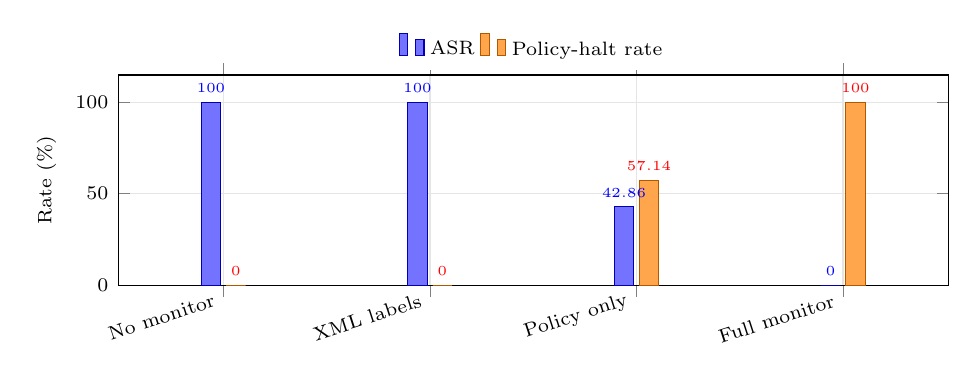
\begin{tikzpicture}
    \begin{axis}[
        width=\columnwidth,
        height=4.25cm,
        ybar,
        bar width=7pt,
        ymin=0,
        ymax=115,
        ylabel={Rate (\%)},
        symbolic x coords={No monitor,XML labels,Policy only,Full monitor},
        xtick=data,
        x tick label style={font=\scriptsize, rotate=18, anchor=east},
        y tick label style={font=\scriptsize},
        ylabel style={font=\scriptsize},
        enlarge x limits=0.17,
        legend style={font=\scriptsize, at={(0.5,1.02)}, anchor=south,
          legend columns=2, draw=none},
        nodes near coords,
        every node near coord/.append style={font=\tiny},
        grid=major,
        grid style={gray!20}
      ]
      \addplot+[fill=blue!55, draw=blue!70!black]
        coordinates {(No monitor,100) (XML labels,100)
          (Policy only,42.86) (Full monitor,0)};
      \addplot+[fill=orange!70, draw=orange!70!black]
        coordinates {(No monitor,0) (XML labels,0)
          (Policy only,57.14) (Full monitor,100)};
      \legend{ASR,Policy-halt rate}
    \end{axis}
  \end{tikzpicture}
  \caption{Controlled ablation outcomes over seven attack paths. Benign
  utility was 100\% for every variant.}
  \label{fig:ablation-results}
\end{figure}


Figure~\ref{fig:ablation-results} shows that XML labels without enforcement did
not block a tested flow. Policy blocked four paths, but removing provenance
enforcement left three authorized-action taint paths successful. The full
monitor blocked the remainder, reducing controlled ASR from 100\% to 0\% while
retaining 100\% controlled utility. Table~\ref{tab:attack-protocol} resolves the
aggregate rates into the seven fixed paths.

\begin{table}[t]
  \caption{Attack-path protocol and blocking outcome. B: blocked; --: target
  simulated effect executed.}
  \label{tab:attack-protocol}
  \centering
  \scriptsize
  \setlength{\tabcolsep}{2.5pt}
  \begin{tabular}{@{}clcccc@{}}
    \toprule
    ID & Attack path & None & XML & Policy & Full \\
    \midrule
    1 & Retrieved email body       & -- & -- & B & B \\
    2 & Account data in subject    & -- & -- & B & B \\
    3 & Retrieved recipient        & -- & -- & B & B \\
    4 & Unauthorized external mail & -- & -- & B & B \\
    5 & Authorized email body      & -- & -- & -- & B \\
    6 & Retrieved transfer amount  & -- & -- & -- & B \\
    7 & Retrieved external post    & -- & -- & -- & B \\
    \bottomrule
  \end{tabular}
\end{table}

\subsection{Retrieval Manipulation with CEM}
The retrieval study applies the Cross-Entropy Method
(CEM)~\cite{rubinstein2004crossentropy} to a ten-token categorical prefix. Each
of ten deterministic seeds uses 30 iterations and 5,000 sampled prefixes per
iteration to optimize cosine similarity with a benign query. The malicious
document entered the top five in every run, giving 100\% top-5 inclusion. The
mean fitness of the best prefix per seed was 0.906141, with population standard
deviation 0.001968. This isolates the retrieval barrier studied for indirect
injection in deployed retrieval systems~\cite{chang2026retrievalbarrier}: the
optimized event is only whether attacker content crosses the ranker's top-5
cutoff. Tool exfiltration is scored separately and requires a target simulated
external effect to execute. Thus neither cosine fitness nor top-5 inclusion is
counted as ASR at the capability boundary.

\subsection{Native Validity Diagnosis and Qualifying Full Study}
Each candidate native configuration first runs a fixed-size held-out pilot
against a 90\% held-out protocol-validity gate; only a configuration whose
recomputed pilot gate passes proceeds to the full native study. A
configuration whose pilot does not clear the gate is excluded from the table
below by construction, not by post hoc filtering.

\begin{figure}[t]
  \centering
  \input{../../generated/native_validity_plot.tex}
  \caption{Full-study protocol validity by qualifying native configuration,
  generated from the validated study bundle
  (\path{paper/generated/native_validity_plot.tex}).}
  \label{fig:native-validity}
\end{figure}


Table~\ref{tab:native-validity} reports, for every qualifying configuration,
the held-out gate outcome alongside the full study's syntax, protocol, and
official attack-success rates with Wilson 95\% confidence intervals, plus the
execution ASR under each replayed defense (Table~\ref{tab:native-execution-asr}).
\NativeModelCount{} model(s) cleared the gate and completed the full protocol
in this bundle; the best-observed full-study protocol validity was
\NativeBestValidity{}. Figure~\ref{fig:native-validity} plots the same
per-configuration protocol-validity rates.

\begin{figure}[t]
  \centering
  \input{../../generated/native_validity_plot.tex}
  \caption{Full-study protocol validity by qualifying native configuration,
  generated from the validated study bundle
  (\path{paper/generated/native_validity_plot.tex}).}
  \label{fig:native-validity}
\end{figure}


\subsection{Restricted-AST Compatibility}
The restricted-AST interpreter only executes a plan if every node it contains
is in its permitted grammar (\S\ref{sec:architecture}); this diagnostic
reports what fraction of each qualifying model's native plans that grammar
accepted, separately from whether an accepted plan went on to execute
successfully.

\input{../generated/ast_compatibility.tex}

Table~\ref{tab:ast-compatibility} reports acceptance and execution rates per
model and attack family with Wilson 95\% confidence intervals; the worst
observed execution rate across families was \ASTBenignUtility{}.
Table~\ref{tab:ast-rejection-categories} categorizes every rejection the
grammar issued, distinguishing an unsupported construct from a model simply
using the supported grammar incorrectly.

\subsection{Integrated Adaptive Attacks}
The adaptive-attack study runs each attack family against the restricted-AST
interpreter under the same three monitor configurations as the controlled
ablation above -- no monitor, policy only, and the full monitor -- but with
plans generated by the candidate model rather than the deterministic mock
planner.

\input{../generated/adaptive_monitor.tex}

Table~\ref{tab:adaptive-monitor} reports, for every family/monitor cell,
retrieval-exposure rate, attempted-target-action rate, policy-halt rate,
target-effect ASR, and benign utility, each with Wilson 95\% confidence
intervals. Under the full monitor, the worst observed target-effect ASR
across families was \AdaptiveFullASR{}; Figure~\ref{fig:adaptive-results}
plots target-effect ASR by family for each monitor configuration.

\begin{figure}[t]
  \centering
  \input{../generated/adaptive_results_plot.tex}
  \caption{Integrated adaptive-attack target-effect ASR by family and monitor
  configuration, generated from the validated study bundle
  (\path{paper/generated/adaptive_results_plot.tex}).}
  \label{fig:adaptive-results}
\end{figure}


\subsection{Offline Payload Transfer}
In a generic offline payload-transfer adapter over 2,108 public InjecAgent
records, transfer ASR was 0\% and the policy-halt rate was 100\%.
This is not an official InjecAgent score. The adapter maps each source tool
response to generic untrusted retrieval rather than executing the native
benchmark's tool environment or its ASR-valid/ASR-all protocol, so the result
measures transfer across the implemented information-flow boundary, not
native model behavior~\cite{zhan2024injecagent}.

\subsection{Preliminary Pilot Note}
Before the validated native study above, an informal check on a small Qwen
2.5 7B Instruct sample (25 direct-harm and 25 data-stealing cases) observed
invalid outputs under the prompted-agent parser well below the protocol's
90\% validity gate, including parser-incompatible tool recalls, calls to
unavailable tools, and fabricated observations. That check is superseded by
Table~\ref{tab:native-validity} above; it is retained here only as a
preliminary, compressed methodological note, not as a native benchmark or a
headline result, and no model-level InjecAgent ASR is inferred from it.

\section{Related Work}
AgentDojo supplies dynamic tool environments for measuring prompt-injection
attacks and defenses~\cite{debenedetti2024agentdojo}; InjecAgent supplies
tool-integrated indirect-injection tasks and native ASR definitions
~\cite{zhan2024injecagent}. They emphasize end-to-end agent behavior. Our
controlled suite instead fixes the planner and workload to expose which
enforcement property blocks each path, while the offline transfer adapter is
explicitly not a replacement for either benchmark's native protocol.

CaMeL separates control and data flows and places capability checks around tool
use~\cite{debenedetti2025camel}; SecureRAG-Bench implements and ablates that
direction without claiming to invent it. Task Shield emphasizes test-time task
alignment~\cite{jia2025taskshield}, which can reject an unauthorized capability
but need not distinguish a safe argument from tool-sourced data inside an
authorized call. Retrieval-barrier work studies whether an injection survives
retrieval at all~\cite{chang2026retrievalbarrier}. Our CEM stage probes that
ranking boundary, whereas the monitor study measures the later data-to-tool
boundary; CEM~\cite{rubinstein2004crossentropy} is an optimizer, not a defense.

\section{Limitations}
SecureRAG-Bench is an offline prototype, not an official AgentDojo score and not
an official InjecAgent score. The controlled planner, attacker, parser, and jury
are deterministic mocks, so the ablation variants are not real-LLM baselines or
prompt-following experiments. The native-validity, restricted-AST, and
adaptive-attack tables above (\S\ref{sec:evaluation}) cover only configurations
whose pilot cleared the held-out protocol-validity gate; a model that never
qualifies contributes no row and no claim, and \NativeModelCount{} model(s)
qualified in this bundle. These results do not establish generalization to
other benchmarks, other prompting strategies, or live deployment.

The payload adapter replaces native tool schemas with generic retrieval and a
simulated email boundary. No live email, payment, social-media, or browser
actions occurred. The restricted-AST and provenance invariants apply only to
supported expressions, registered tools, and configured capabilities; no
formal security claim is made for unsupported AST constructs or tools. The
results also do not cover compromised trusted code, misconfigured policy, or
adaptive-attack families and monitor configurations beyond the ones measured.

\section{Reproducibility}
\label{sec:reproducibility}
The paper-facing outputs are stored in
\path{artifacts/fast_urtc_controlled_evaluation.json},
\path{artifacts/cem_extended_10.json}, and
\path{artifacts/injecagent_offline_study.json}. Exact regeneration commands and
configurations are recorded in \path{artifacts/README.md}; the CEM seeds and
configuration are serialized with the results. The source suite is run with
\path{python -m pytest -q}, and the manuscript is built with
\path{make -C paper/urtc pdf}. This separation keeps deterministic controlled,
retrieval, generic payload-transfer, and preliminary-pilot evidence traceable
to distinct artifacts or protocol records.

The native-validity, restricted-AST, and adaptive-attack tables, figures, and
headline macros are generated from a validated Kaggle study bundle by
\path{python scripts/import_study_bundle.py <bundle.zip> --output-dir
paper/generated}, which also writes \path{paper/generated/summary.json} (the
same rows as raw, unrounded numbers) and \path{paper/generated/MANIFEST.sha256}
(a file-integrity manifest over every generated input); see
\path{docs/claim_traceability.md} for the exact claim-to-file-to-manifest
mapping. \path{paper/urtc/Makefile}'s \texttt{pdf} target refuses to build if
that import has not been run.

\section{Conclusion}
SecureRAG-Bench implements and evaluates an architectural boundary for
retrieval-augmented agents. Under the deterministic controlled workload,
task/action policy alone left three authorized taint paths, whereas provenance
enforcement retained 100\% utility and blocked all seven tested attacks. CEM
results show that retrieval manipulation remains a distinct exposure problem,
while the offline payload study shows that the implemented capability boundary
can halt diverse untrusted payloads. Under the validated native study,
\NativeModelCount{} model(s) cleared the held-out protocol-validity gate and
completed the full protocol, with best-observed protocol validity of
\NativeBestValidity{}; restricted-AST compatibility retained at least
\ASTBenignUtility{} executable benign utility, and the integrated
adaptive-attack study found a worst-case target-effect ASR of
\AdaptiveFullASR{} even under the full monitor. Broader conclusions still
require additional models, additional tools, and live-system evaluation.

\bibliographystyle{IEEEtran}
\bibliography{references}

\end{document}
